\documentclass[10pt,a4paper]{article}
\usepackage[utf8]{inputenc}
\usepackage{amsmath}
\usepackage{amsfonts}
\usepackage{graphicx}
\usepackage{amssymb}
\author{Brian Lauer}

\begin{document}

\begin{figure}
\centering
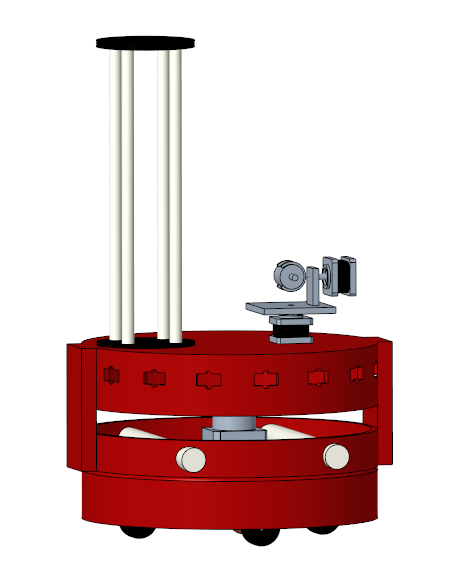
\includegraphics[scale=0.5]{figs/img/frontViewScreenshotB}
\caption{Current cleaning, disinfection, and mapping robot design}
\label{camRobot}
\end{figure}

Many different robots exist on the market for the purpose of UV disinfection from companies like UVD Robots. These robots typically employ sensors like ultrasonic sensors for ranging, LIDAR sensors or cameras for generation of a digital map of a room, and cliff sensors for recognition of drops or edges. One of the main features they employ is a UVC lamp that is capable of performing efficient elimination of many harmful microorganisms including bacteria and viruses within a room through DNA destruction and disruption. However, a limitation to these current robots on the market is the inability to shine UV light vertically: only horizontally with full 360$^\circ$ range of emission. The proposed robot design shown in Figure \ref{camRobot} will support emission of light horizontally as well as vertically by including two horizontally positioned lamps able to disinfect areas directly above the robot. Secondly, because UV light is deemed dangerous to humans and possibly other animals a disinfection sprayer will help to further reduce the concentration of harmful pathogens. In this way, full room disinfection can be accounted for in case any live animals are unable to be relocated during the disinfection period. During disinfection of a room with UVC light such as a hospital room, no humans or animals may be present. To provide a maximum turning radius and stability, the robot features a two-wheel differential drive design with two additional points of contact via two caster wheels. For creation of a digital map, a LIDAR sensor is present in the center of the robot which will relay serial data to the robot's central computer, a Beaglebone single board computer with the SLAM (Simultaneous Localization and Mapping) algorithm.

Another feature that the proposed robot will boast is the presence of a vacuuming mechanism capable of removing dust particles or debris from floor surfaces. In this way, a room can be thoroughly cleaned with little to no human intervention which is in favor due to the current health crisis. This robot will be able to effectively combine the features of the robot designs by iRobot and UVD robots. Another feature that this robot will propose to implement is the integration of a mobile application capable of wireless communication with the onboard computer of the robot to direct the robot to perform various actions like directing the robot to a specific room or area of a home or building. Secondly, a real time 2D map of the room will be visible to allow owners to view the current progress of the cleaning and disinfection process. Lastly, 14 ultrasonic sensors will be present around the circumference of the robot chassis to perform additional ranging and obstacle avoidance.
\end{document}